\documentclass[../main.tex]{subfiles}

\usepackage{graphicx}
\graphicspath{ {fig/count/} }

\title{Discrete}
\author{}
\date{}

\begin{document}

\maketitle
\tableofcontents

\newpage

\section{Counting}

\subsection{Permutations, Combinations}

Suppose we want to find how many ways we can arrange
\( n \) objects in \( r \) positions, with \( n \geq r \).
To find this, first consider the case when \( n = r \).
There are \( n \) choices of objects to put in the first position, then \( n - 1 \) and so on.
So the number of ways to arrange \( n \) objects in \( n \) positions is just \( n! \).
Put another way,
we want to know how many ways we can map each position to one object.
This is the number of bijections or permutations of \( n \) objects.

\noindent
\begin{tikzpicture}[x=0.75pt,y=0.75pt,yscale=-1,xscale=1]
%uncomment if require: \path (0,300); %set diagram left start at 0, and has height of 300

%Shape: Axis 2D [id:dp791486377406529] 
\draw  (50,241.7) -- (314.5,241.7)(76.45,41) -- (76.45,264) (307.5,236.7) -- (314.5,241.7) -- (307.5,246.7) (71.45,48) -- (76.45,41) -- (81.45,48) (115.45,236.7) -- (115.45,246.7)(154.45,236.7) -- (154.45,246.7)(193.45,236.7) -- (193.45,246.7)(232.45,236.7) -- (232.45,246.7)(271.45,236.7) -- (271.45,246.7)(71.45,202.7) -- (81.45,202.7)(71.45,163.7) -- (81.45,163.7)(71.45,124.7) -- (81.45,124.7)(71.45,85.7) -- (81.45,85.7) ;
\draw   ;
%Curve Lines [id:da6119806462814916] 
\draw    (76.45,241.7) .. controls (112.5,67) and (290.5,90) .. (292.5,82) ;
%Shape: Axis 2D [id:dp1956952642703632] 
\draw  (370,238.7) -- (634.5,238.7)(396.45,38) -- (396.45,261) (627.5,233.7) -- (634.5,238.7) -- (627.5,243.7) (391.45,45) -- (396.45,38) -- (401.45,45) (435.45,233.7) -- (435.45,243.7)(474.45,233.7) -- (474.45,243.7)(513.45,233.7) -- (513.45,243.7)(552.45,233.7) -- (552.45,243.7)(591.45,233.7) -- (591.45,243.7)(391.45,199.7) -- (401.45,199.7)(391.45,160.7) -- (401.45,160.7)(391.45,121.7) -- (401.45,121.7)(391.45,82.7) -- (401.45,82.7) ;
\draw   ;
%Curve Lines [id:da6904688712857534] 
\draw    (396.45,238.7) .. controls (432.5,64) and (610.5,87) .. (612.5,79) ;
%Straight Lines [id:da8868203342962732] 
\draw [color={rgb, 255:red, 255; green, 0; blue, 0 }  ,draw opacity=1 ]   (396.45,238.7) -- (429.5,159) ;
%Straight Lines [id:da6732443966151707] 
\draw [color={rgb, 255:red, 255; green, 0; blue, 0 }  ,draw opacity=1 ]   (429.5,159) -- (494.5,105) ;
%Straight Lines [id:da792722354522738] 
\draw [color={rgb, 255:red, 255; green, 0; blue, 0 }  ,draw opacity=1 ]   (600.5,81) -- (494.5,105) ;
%Straight Lines [id:da7780337638207823] 
\draw [color={rgb, 255:red, 0; green, 42; blue, 255 }  ,draw opacity=1 ]   (429.5,159) -- (493.5,159) ;
%Straight Lines [id:da5469718819271276] 
\draw [color={rgb, 255:red, 0; green, 42; blue, 255 }  ,draw opacity=1 ]   (493.5,159) -- (493.5,107) ;

% Text Node
\draw (42,139.4) node [anchor=north west][inner sep=0.75pt]    {$y$};
% Text Node
\draw (174,263.4) node [anchor=north west][inner sep=0.75pt]    {$x$};
% Text Node
\draw (362,136.4) node [anchor=north west][inner sep=0.75pt]    {$y$};
% Text Node
\draw (494,260.4) node [anchor=north west][inner sep=0.75pt]    {$x$};
% Text Node
\draw (454,167.4) node [anchor=north west][inner sep=0.75pt]  [color={rgb, 255:red, 0; green, 95; blue, 255 }  ,opacity=1 ]  {$dx$};
% Text Node
\draw (504,126.4) node [anchor=north west][inner sep=0.75pt]  [color={rgb, 255:red, 0; green, 24; blue, 255 }  ,opacity=1 ]  {$dy$};
% Text Node
\draw (407,75.4) node [anchor=north west][inner sep=0.75pt]  [color={rgb, 255:red, 255; green, 0; blue, 0 }  ,opacity=1 ]  {$\sqrt{dx^{2} +dy^{2}}$};


\end{tikzpicture}

Now consider \( n > r \).
We want the number of ways we can map each position to one object.
This is the number of injections from \( r \) to \( n \).
To find this, imagine we have \( n \) positions again,
but we don't care about the positions after \( r \).
We can consider any two arrangements to be equivalent,
as long as the first \( r \) positions are the same.
We can "quotient" out the redundant arrangements by how many there are.
Thus, we get
\[ P(n, r) = \frac{n!}{(n - r)!}. \]

Likewise,
if we don't care about the order of the objects in the first \( r \) positions,
we can consider all arrangements that have the same objects in those positions
to be equivalent,
and quotient out the number of redundant arrangements.
Thus, the number of combinations is
\[ C(n, r) = \binom{n}{r} = \frac{n!}{r! (n - r)!}. \]

Now, suppose we have \( n \) objects and \( r \) positions with \( n > r \).
We want to figure out how many ways there are to put all the objects into the positions.
This is the number of mappings from \( n \) to \( r \).
For each object, we map it to a position.
We find this by \( r^n \).

\subsection{Pascal's Triangle}

Imagine a triangle of numbers arranged such that each number is the sum of the two above it.

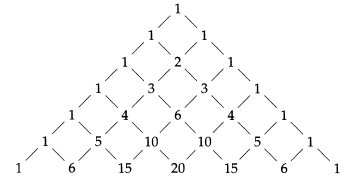
\includegraphics{2.png}

One convenient way to think about the number \( n \) rows down and \( r \) columns right
is to think about how many paths there are to that position from the top.
We know the path has to be \( n \) long and composed of left and right turns.
It must also have \( r \) right turns.

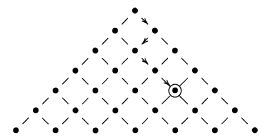
\includegraphics{3.png}

Therefore, the number of paths is just the ways we can choose \( r \) right turns
out of \( n \) total turns, or \( \binom{n}{r} \).

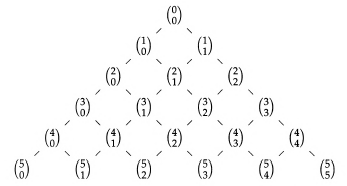
\includegraphics{4.png}

Then it is easy to see that the total number of paths at \( (n, r) \)
is just the sum of the number of paths to the nodes above it,
or \( \binom{n}{r} = \binom{n - 1}{r - 1} + \binom{n - 1}{r} \)
which is also known as Pascal's Identity.

\subsubsection{Hockey Stick Identity}

Suppose we want to find
\[ \sum_{k=r}^n \ = \binom{r}{r} + \binom{r+1}{r} +
\dots
+ \binom{n-1}{r} + \binom{n}{r}. \]
If we examine the triangle,
we have all the nodes along a diagonal starting from \( \binom{r}{r} \).
Let's examine the node \( \binom{n+1}{r+1} \).
We know this is just the sum of the nodes above it,
so \( \binom{n}{r} + x_1 \).
But \( x_1 \) is just the sum of the nodes above it, so \( \binom{n-1}{r} + x_2 \).
Continuing this way, we can see that
\[ \sum_{k=r}^n \binom{k}{r} = \binom{n+1}{r+1}. \]

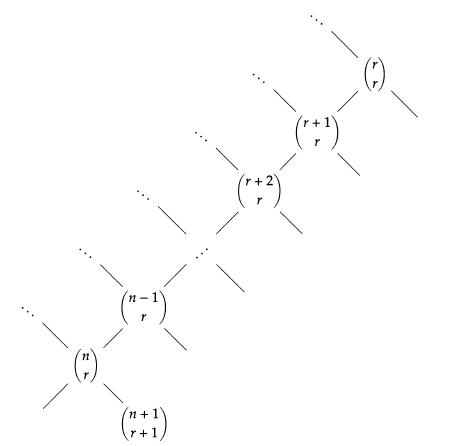
\includegraphics{5.png}



\subsection{Binomial Theorem}

Take \[ (a + b)^n = \underbrace{(a + b)(a + b)\dots(a + b)}_n. \]
We must go through every combination of \( a \) and \( b \).
From each term,
we must choose either \( a \) or \( b \), and there are \( n \) terms in total.
Then the number of ways to choose \( r \) amount of \( b \)s out of \( n \) terms
is just \( \binom{n}{r} \).
\begin{align*}
    (a + b)^n &= \binom{n}{0} a^n + \binom{n}{1} a^{n-1}b + \binom{n}{2} a^{n-2}b^2 +
    \dots
    + \binom{n}{n-1} ab^{n-1} + \binom{n}{n} b^n \\
    &= \sum_{r = 0}^n \binom{n}{r} a^{n-r} b^r.
\end{align*}



\section{Number Theory}

\subsection{Primes}

Primes numbers are like atoms of natural numbers.
Composite numbers can be broken down into divisors repeatedly,
until all divisors are prime themselves and are no longer divisible.
By the Fundamental Theorem of Arithmetic,
all natural numbers have a unique prime factorization.

The Sieve of Eratosthenes is an algorithm for differentiating primes and composites.
It works by starting with the smallest prime, 2,
then eliminating all multiples of it.
Next, go to the next highest number not eliminated.
This will be a prime, since none of the lower numbers were divisors.
Continuing this way, we eventually find all primes.

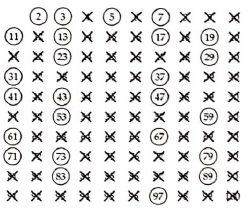
\includegraphics{fig/num/1.png}

Note that when we are at a certain prime and eliminate a multiple as composite,
this is the smallest prime divisor of that number.


\end{document}